\documentclass[a4paper]{article}

\usepackage[inline]{enumitem}
\usepackage{xcolor}
\usepackage{fontspec}
\usepackage[english, russian]{babel}

% download "Linux Libertine" fonts:
% http://www.linuxlibertine.org/index.php?id=91&L=1
\setmainfont{Linux Libertine O} % or Helvetica, Arial, Cambria
% why do we need \newfontfamily:
% http://tex.stackexchange.com/questions/91507/
\newfontfamily{\cyrillicfonttt}{Linux Libertine O}





\usepackage{amsmath} % Математические окружения AMS
\usepackage{amsfonts} % Шрифты AMS
\usepackage{amssymb} % Символы AMS
\usepackage{mathtext} % Русские буквы в фомулах
\usepackage{graphicx} % Вставить pdf- или png-файлы

\usepackage{color}
\usepackage{bbold}

\usepackage{booktabs}

\usepackage{mathrsfs} % Красивый шрифт

\usepackage{longtable}  % Длинные таблицы
\usepackage{multirow} % Слияние строкв таблице

\usepackage{indentfirst} % Отступ в первом абзаце.
\usepackage{tikz}

\newcommand*{\hm}[1]{#1\nobreak\discretionary{}%
            {\hbox{$\mathsurround=0pt #1$}}{}}

\usepackage{verbatim}

\DeclareMathOperator{\sgn}{\mathop{sgn}}
\DeclareMathOperator{\card}{\mathop{card}}

\usepackage{enumitem}


\usepackage{fancyhdr}
\usepackage[margin=1in]{geometry}


\AddEnumerateCounter{\asbuk}{\russian@alph}{щ} % для списков с русскими буквами
\setlist[enumerate, 2]{label=\asbuk*),ref=\asbuk*}


\pagestyle{fancy} \makeatletter \fancyhead[L]{\footnotesize ICEF, 2016/17, «Mathematics for Economists»}

\makeatletter
\newcommand*{\rom}[1]{\expandafter\@slowromancap\romannumeral #1@}
\makeatother

\linespread{1.5}
 \begin{document}
 \begin{center}
 {\Large{Конспект лекции 29.11.16}}
 \end{center}
 \par {\bf\underline{Интуиция (теорема об остановке мартингала):}} Если ${M}_t$ (мартингал) $\equiv$ справедливая игра \\ То есть, если \begin{enumerate*}[label={\alph*)},font={\color{red!50!black}\bfseries}] \item Правило входа из игры не "заглядывает" в будущее \item Ставки не растут слишком быстро (технические условия теоремы А,Б,В) \end{enumerate*} то $E({M}_\tau)$=$E({M}_1)$, то есть ожидаемый выигрыш на момент выхода равен стартовому благосостоянию (невозможно повысить или понизить начальное благосостояние)
 \\
 \par {\bf\underline{Упражнение 1:}}
\begin{figure}[h]
\center{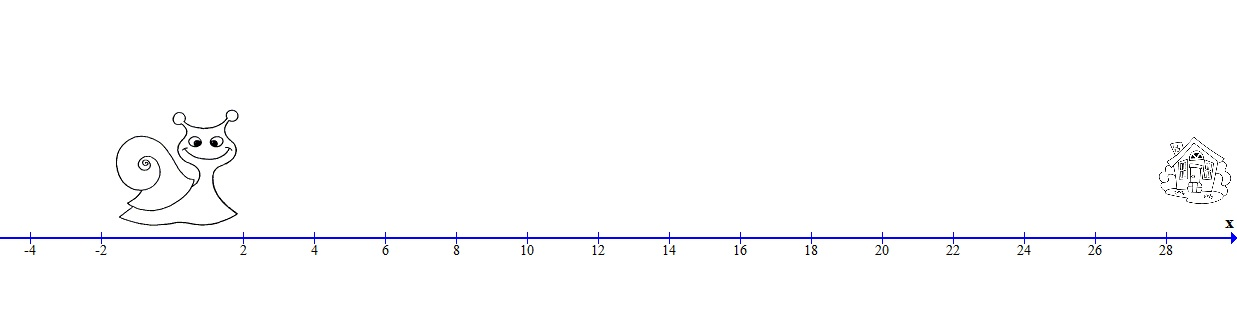
\includegraphics[width=1\linewidth]{03_home.jpg}}
\label{image}
\end{figure}
В начальный момент времени улитка находится в точке с координатой ''$0$''. Она может передвигаться на один шаг вправо или влево в каждую следующую единицу времени. Ее передвижения ограничены: в точке с координатой ''$-5$'' находится пропасть, а в точке с координатой ''$30$'' -- ее дом.
 Ходы улитки независимы друг от друга. \\
 Введем процесс $({X}_t)$ -- координата улитки в момент времени $t$ и: \begin{enumerate*}[font={\color{red!50!black}\bfseries}] \item ${X}_0=0$; \item ${X}_t={Z}_1+{Z}_2+\dots+{Z}_t$ \end{enumerate*}, где ${Z}_i$ - случайная величина, отвечающая за перемещение улитки (влево или вправо соответственно) в момент $i$, распределение которой может быть представлено следующим образом:
\begin{table}[h]
\centering
\begin{tabular}{l|c|c}
${Z}_i$ & $-1$ & $1$ \\ \hline
$p$ & $\frac{1}{4}$ & $\frac{3}{4}$
\end{tabular}
\end{table}
(${Z}_i=-1$ -- движение влево, ${Z}_i=1$ -- вправо)
\begin{enumerate}[label={\alph*)}]
\item $({X}_t)$ -- мартингал?\\
Проверка по определению: $E({X}_{t+1}|\mathcal{F}_t)=E({X}_t+{Z}_{t+1}|\mathcal{F}_t)={X}_t+E({Z}_{t+1}|\mathcal{F}_t)={X}_t+E({Z}_{t+1})={X}_t+\frac{1}{2}\neq{X}_t $
\\ Замечание: $\mathcal{F}_t= \sigma({Z}_1,{Z}_2,\dots,{Z}_t)$ и так как ходы независимы, то есть ${Z}_{t+1}$ не зависит от ${Z}_1,{Z}_2,\dots,{Z}_t$, то $E({Z}_{t+1}|\mathcal{F}_t)=E({Z}_{t+1})$
\\ Ответ: Нет
\item Найти такое $b$, что ${Y}_t={X}_t-b*t$ будет мартингалом \\
По определению мартингала нужно получить: $E({Y}_{t+1}|\mathcal{F}_t)={Y}_t$
\\ $E({Y}_{t+1}|\mathcal{F}_t)=E({X}_{t+1}-b*(t+1)|\mathcal{F}_t)={X}_t+\frac{1}{2}-b*t-b={Y}_t+\frac{1}{2}-b \Rightarrow b=\frac{1}{2}$
\item  Найти такое $c\neq{1}$, что ${R}_t=c^{{X}_t}$ будет мартингалом
\\ Аналогично предыдущему пункту:$E({R}_{t+1}|\mathcal{F}_t)={R}_t$
\\ $E({R}_{t+1}|\mathcal{F}_t)=E(c^{{X}_{t+1}}|\mathcal{F}_t)=E(c^{{X}_t+{Z}_{t+1}}|\mathcal{F}_t)=c^{{X}_t}*E(c^{{Z}_{t+1}|\mathcal{F}_t})=c^{{X}_t}*E(c^{{Z}_{t+1}})=c^{{X}_t}*(\frac{1}{4}*c^{-1}+\frac{3}{4}*c)={R}_t=c^{{X}_t} \Rightarrow \frac{1}{4}*c^{-1}+\frac{3}{4}*c=1 \Rightarrow  3*c^2-4*c+1=0 \Rightarrow {c}_1=1,{c}_2=\frac{1}{3}$
\\ Ответ: ${R}_t={\frac{1}{3}}^{{X}_t}$
\item $Pr(\text{улитка дойдет до точки ''30''})=?$
\\ Введем момент остановки: $\tau=\min(t|{X}_t=30 \ \text{или} \ {X}_t=-5)$
\\ Для мартингала из пункта b) по теореме об остановке мартинагала: $E({Y}_{\tau})=E({Y}_{1})=E({X}_{1}-\frac{1}{2})=\frac{1}{2}-\frac{1}{2}=0$
\\В то же время $E({Y}_{\tau})=E({X}_{\tau}-\frac{1}{2}*\tau)=E({X}_{\tau})-\frac{1}{2}*E(\tau)=0$
\\Аналогично для мартингала из пункта с): $E({R}_{\tau})=E({R}_{1})=E({\frac{1}{3}}^{{X}_{1}})=\frac{1}{4}*{\frac{1}{3}}^{-1}+\frac{3}{4}*\frac{1}{3}=1$
\\В то же время $E({R}_{\tau})=E({\frac{1}{3}}^{{X}_{\tau}})=1$
\\ При этом ${X}_{\tau}$ -- случайная величина, координата конечной точки улитки:
\begin{table}[h]
\centering
\begin{tabular}{l|c|c}
${X}_{\tau}$ & $30$ & $-5$ \\ \hline
$p$ & $k$ & $1-k$
\end{tabular}
\end{table}
\\ Где ''$k$'' -- искомая вероятность
\\ Таким образом, $E({R}_{\tau})=E({\frac{1}{3}}^{{X}_{\tau}})=k*{\frac{1}{3}^{30}}+(1-k)*{\frac{1}{3}^{-5}}=1 \Rightarrow k*{3^{-30}}+(1-k)*{3^{5}}=1 \Rightarrow k*({3^{5}}-{3^{-30}})=3^{5}-1 \Rightarrow k\approx0.996$
\\ Ответ:  $Pr(\text{улитка дойдет до точки ''30''})=0.996$
\item Определить ожидаемое количество шагов до одной из конечных точек
\\ Из предыдущего пункта знаем, что $E({X}_{\tau})-\frac{1}{2}*E(\tau)=0 \Rightarrow E({X}_{\tau})=30*k-5*(1-k)=30*0.996-5*0.004=\frac{1}{2}*E(\tau) \Rightarrow E(\tau)=2*E({X}_{\tau})=60*0.996-10*0.004=59.72$
\\ Ответ: ожидаемое количество шагов до одной из конечных точек -- $59.72$
\end{enumerate}
\par {\bf\underline{Упражнение 2 (Задача о мартышке):}} Мартышка нажимает кнопки на клавиатуре случайным образом, делая одно нажатие в секунду. Пусть $\tau$ -- момент первого написания мартышкой слова ''AБРАКАДАБРА''. Найдите $E(\tau)$.
\\Решение: необходимо придумать мартингал. \\ Пусть существует ''казино'' в котором можно делать ставки на следующую букву, набранную мартышкой. Действуют следующие правила: \begin{enumerate*}[font={\color{red!50!black}\bfseries}] \item Если $s$ -- ставка, то в случае угадывания выигрыш составляет $33*s$, в случае проигрыша $-s$; \ \item Каждая следующая ставка равна всему предыдущему благосостоянию игрока (то есть все имеющиеся деньги ставятся на следующую букву); \ \item В каждый момент времени в ''казино''приходит один новый игрок со стартовым благосостоянием равным одному рублю. \end{enumerate*}
\\ Пусть $({Y}_{t})$ -- суммарное благосостояние всех игроков. $E({Y}_{1})=1, E({Y}_{2})=2, E({Y}_{3})=3 \dots E({Y}_{t})={Y}_{t} \Rightarrow$ можно получить мартингал из  $({Y}_{t})$:  $({Z}_{t})=({Y}_{t}-t)$ (проверка по определению)
\\ Можем применить теорему об остановке мартингала: $E({Z}_{\tau})=E({Z}_{1})=0, \ \text{в то же время} \ E({Z}_{\tau})=E({Y}_{\tau}-\tau) \Rightarrow E({Y}_{\tau}-\tau)=0 \Rightarrow E({Y}_{\tau})= E(\tau)$ \\
Предположим теперь, что каждый игрок делает ставки последовательно на каждую букву слова "АБРАКАДАБРА". Тогда в момент $\tau$ суммарное благосостояние всех игроков состоит из \begin{enumerate*}[font={\color{red!50!black}\bfseries}] \item благосостояния игрока который пришел в тот момент, когда мартышка начала писать слово и правильно угадал все 11 букв; \item благосостояния игрока, который пришел в момент  $\tau$; \item благосостояния игрока который пришел на восьмой букве слова и правильно угадал четыре буквы до момента $\tau$ \end{enumerate*}. Все остальные игроки остались с $0$ выигрышем. Таким образом, ${Y}_{\tau}=33^{11}+33^4+33 \Rightarrow E({Y}_{\tau})={Y}_{\tau}=33^{11}+33^4+33=5.05*{\exp}^{16} =E(\tau)$
\\ Ответ: $E(\tau)=5.05*{\exp}^{16}$ (очень большое, но конечное значение)
\\ \par {\bf\underline{Непрерывное время}} $t\in[0;+\infty)$
\par {\bf\underline{Определение}} Фильтрация $({\mathcal{F}_{t}})_{t\in[0;+\infty)}$ -- упорядоченное множество $\sigma$-алгебр $\mathcal{F}_{s} \subseteq \mathcal{F}_{t}$ при $s\leq t$
\par {\bf\underline{Определение}} Случайный процесс $({X}_t)$ -- мартингал по отношению к фильтрации $({\mathcal{F}_{t}})$, если \begin{enumerate}
 \item Существует $E({X}_{t})$ $\forall t$
 \item ${X}_t$ является ${\mathcal{F}_{t}}$-измеримой $\forall t$
 \item $E({X}_{t+\delta}|{\mathcal{F}_{t}})={X}_{t} \ \forall t, \ \delta \geq 0$
 \end{enumerate}
\par {\bf\underline{Определение}} $({W}_t)$ -- винеровский процесс (или броуновское движение) по отношению к фильтрации $({\mathcal{F}_{t}})$, если
 \begin{enumerate}
 \item  ${W}_0=0$
 \item  $Pr(\text{траектория ${W}_t$ непрерывна})=1$
 \item  Для двух моментов времени $s\ \text{и}\ t, s \geq 0, s<t, {W}_t-{W}_s$ не зависит от $\mathcal{F}_{s}$
 \item ${W}_t-{W}_s \sim \mathcal{N}(0,t-s)$
 \item ${W}_t$ -- измерима относительно $({\mathcal{F}_{t}})$
 \end{enumerate}
\par {\bf\underline{Альтернативное определение}}
\begin{enumerate}
 \item  ${W}_0=0$
 \item  $Pr(\text{траектория ${W}_t$ непрерывна})=1$
 \item  Случайные величины ${W}_{t_1}-{W}_{s_1}, {W}_{t_2}-{W}_{s_2} \dots$ -- независимы
 \item  ${W}_t-{W}_s \sim \mathcal{N}(0,t-s)$
 \end{enumerate}
\par {\bf\underline{Упражнение 3}}  ${W}_t$ -- винеровский процесс. Найдите: \begin{enumerate*}[font={\color{red!50!black}\bfseries}] \item $E({W}_t)$ \item $E({{W}^2}_t)$ \item $E({{W}^3}_t)$  \item $E({W}_t*{W}_s)$ \item $\text{Cov}[{W}_t,{W}_s]$ \item $\text{Corr}[{W}_t,{W}_s]$ \item $({W}_t)$ -- мартингал?  \item $({{W}^2}_t-t)$ -- мартингал? \item $Pr({W}_7>9*{W}_4)$ \item $Pr(\lvert {W}_{100}\rvert >20)$ \end{enumerate*}
\\ Решение:
\begin{enumerate}
\item $E({W}_t)=E({W}_t-{W}_s)=E({W}_t-{W}_0)=E({W}_t-0)$ (Примечание: поскольку $s$ -- произвольное, то выбираем его равным $0$ и применяем свойства $1.$ и $4.$ из определения)
\item $E({{W}^2}_t)=\text{Var}({W}_t)=t-s=t-0=t$
\item $E({{W}^3}_t)=\int_{-\infty}^{+\infty} w^3 * f(w) dw = 0 $
\item Для $s<t$: $E({W}_t*{W}_s)=\text{Cov}[{W}_s+\delta, {W}_s]=\text{Cov}[{W}_s, {W}_s]+ \text{Cov}[\delta,{W}_s]=\text{Var}({W}_s)=s$ (Примечание: $\delta={W}_t-{W}_s$, по свойству 3. определения ${W}_t-{W}_s$ не зависит от $\mathcal{F}_{s}$, а значит $\text{Cov}[\delta,{W}_s]=\text{Cov}[{W}_t-{W}_s,{W}_s]=0$)
\\ Аналогично для $s>t$: $E({W}_t*{W}_s)=t \Rightarrow$ в общем случае $E({W}_t*{W}_s)=\text{min}[s,t]$
\item $\text{Cov}[{W}_t,{W}_s] =E({W}_t*{W}_s)-E({W}_t)*E({W}_s)=\text{min}[s,t]-0*0=\text{min}[s,t]$
\item $\text{Corr}[{W}_t,{W}_s]=\frac{\text{Cov}[{W}_t,{W}_s]}{ \sqrt{\text{Var}({W}_s)}*\sqrt{\text{Var}({W}_t)}}=\frac{\text{min}[s,t]}{\sqrt{t*s}}$
\item Проверка по определению: $E({W}_{t+\delta}|{\mathcal{F}_{t}})=E({W}_{t+\delta}+{W}_{t}-{W}_{t}|{\mathcal{F}_{t}})={W}_{t}+E({W}_{t+\delta}-{W}_{t}|{\mathcal{F}_{t}})={W}_{t} \Rightarrow$ $({W}_{t})$ -- мартингал. (Примечание: $E({W}_{t+\delta}-{W}_{t})=0$ по свойству 4. определения)
\item  Проверка по определению: $E({W^2}_{t+\delta}-t-\delta|{\mathcal{F}_{t}})=-t-\delta+E({W^2}_{t+\delta}|{\mathcal{F}_{t}})=-t-\delta+E(({W}_{t}+({W}_{t+\delta}-{W}_{t}))^2|{\mathcal{F}_{t}})=-t-\delta+{{W}^2}_t + 2{W}_{t}*E({W}_{t+\delta}-{W}_{t})+E(({W}_{t+\delta}-{W}_{t})^2)=-t-\delta+{{W}^2}_t+\text{Var}({W}_{t+\delta}-{W}_{t})={{W}^2}_t-t \Rightarrow$ \ $({{W}^2}_t-t)$ -- мартингал
\item $Pr({W}_7>9*{W}_4)=Pr({W}_7-9*{W}_4>0)=Pr(({W}_7-{W}_4) - 8*{W}_4>0)$ \\ ${W}_7-{W}_4 \sim \mathcal{N}(0,3)$, $8*{W}_4 \sim \mathcal{N}(0,64*4)\Rightarrow \text{Var}(({W}_7-{W}_4) - 8*{W}_4)=64*4+3=259 \Rightarrow ({W}_7-{W}_4) - 8*{W}_4 \sim \mathcal{N}(0,259) \Rightarrow Pr(({W}_7-{W}_4) - 8*{W}_4>0)=\frac{1}{2} $
\item $Pr(\lvert {W}_{100}\rvert >20)=Pr(\frac{\lvert {W}_{100}\rvert}{10} >2)$
\\ ${W}_{100} \sim \mathcal{N}(0,100) \Rightarrow \frac{\lvert {W}_{100}\rvert}{10} \sim \mathcal{N}(0,1) \Rightarrow =Pr(\frac{\lvert {W}_{100}\rvert}{10} >2)\approx0.05$
\end{enumerate}
\end{document}
